% Cahier des charges — Projet PMD2 CT-CORA3D (ECAM, Master en ingénierie biomédicale)
% Compilateur Overleaf : pdfLaTeX (Menu → Compiler).
\documentclass[11pt,a4paper]{article}

\usepackage[utf8]{inputenc}
\usepackage[T1]{fontenc}
\usepackage[french]{babel}
\usepackage{lmodern}
\usepackage[margin=2.3cm]{geometry}
\usepackage{graphicx}
\usepackage{xcolor}
\usepackage{tabularx}
\usepackage{booktabs}
\usepackage{longtable}
\usepackage{enumitem}
\usepackage{tikz}
\usetikzlibrary{arrows.meta,positioning}
\usepackage{fancyhdr}
\usepackage{titlesec}
\usepackage[hidelinks]{hyperref}

\definecolor{ecam}{RGB}{30,60,140}
\titleformat{\section}{\Large\bfseries\color{ecam}}{\thesection.}{0.6em}{}
\titleformat{\subsection}{\large\bfseries\color{ecam}}{\thesubsection}{0.6em}{}
\setlist{itemsep=2pt}
\renewcommand{\arraystretch}{1.25}

\pagestyle{fancy}
\fancyhf{}
\lhead{\small Cahier des charges — CT-CORA3D}
\rhead{\small Projet PMD2 · ECAM}
\cfoot{\thepage}

\newcommand{\exigence}[3]{\textbf{#1} & #2 & #3 \\ \midrule}

\begin{document}

% ------------------------------------------------------------------ page de titre
\begin{titlepage}
  \centering
  
\includegraphics[width=0.38\textwidth]{images/logo_ecam.png}\par\vspace{2.5cm}
  {\Huge\bfseries\color{ecam} Cahier des charges\par}\vspace{0.6cm}
  {\LARGE CT-CORA3D\par}\vspace{0.3cm}
  {\large Planification 3D des ostéotomies de correction de la patte arrière du chien\\ et guides chirurgicaux imprimés en 3D\par}
  \vfill
  {\large Projet PMD2 — Master en ingénierie biomédicale\par}\vspace{0.3cm}
  {\large Groupe : \textit{(noms des membres du groupe)}\par}\vspace{0.3cm}
  {\large Année académique 2026–2027\par}\vspace{0.3cm}
  {\large Version 1.0 — \today\par}
\end{titlepage}

\tableofcontents
\newpage

% ------------------------------------------------------------------ 1
\section{Contexte et objectif}

Certains chiens présentent des déformations des os longs de la patte arrière (fémur, tibia) : l'os est penché, arqué
ou tordu, ce qui fait boiter l'animal et use ses articulations (luxation de la rotule, arthrose du genou). Le traitement est une \textbf{ostéotomie de correction} : le
chirurgien coupe l'os à l'endroit de la déformation, le remet droit, puis le fixe avec une plaque.

La difficulté est de savoir \textbf{où} couper, \textbf{de combien} corriger et \textbf{comment} reproduire ce plan
pendant l'opération. La méthode de référence est la \textbf{méthode du CORA} (Paley), habituellement appliquée sur des
radiographies 2D, ce qui est imprécis quand la déformation est oblique ou tordue.

\paragraph{Objectif du projet.} Développer une chaîne logicielle qui, à partir du scanner (CT) du chien :
\begin{enumerate}
  \item reconstruit les os en 3D ;
  \item mesure la déformation et planifie la correction en 3D (méthode du CORA) ;
  \item conçoit deux guides chirurgicaux sur mesure, imprimables en 3D : un \textbf{guide de coupe} et un
        \textbf{guide de réduction}.
\end{enumerate}

\begin{figure}[h]
  \centering
  \begin{tikzpicture}[node distance=0.55cm, every node/.style={font=\small},
      etape/.style={draw=ecam, thick, rounded corners, fill=ecam!8, align=center, minimum height=1.1cm, text width=2.3cm},
      fleche/.style={-{Stealth}, thick, ecam}]
    \node[etape] (a) {Scanner\\(DICOM)};
    \node[etape, right=of a] (b) {Os en 3D\\(segmentation)};
    \node[etape, right=of b] (c) {Repères\\anatomiques};
    \node[etape, right=of c] (d) {Planification\\CORA 3D};
    \node[etape, right=of d] (e) {Guides\\imprimables};
    \draw[fleche] (a) -- (b); \draw[fleche] (b) -- (c); \draw[fleche] (c) -- (d); \draw[fleche] (d) -- (e);
  \end{tikzpicture}
  \caption{Chaîne de traitement de CT-CORA3D.}
\end{figure}

% ------------------------------------------------------------------ 2
\section{Périmètre du projet}

\begin{tabularx}{\textwidth}{@{}XX@{}}
\toprule
\textbf{Inclus} & \textbf{Hors périmètre} \\ \midrule
Lecture des scanners DICOM & Réalisation de la chirurgie \\
Segmentation et identification des os de la patte arrière (fémur, tibia, fibula, rotule) & Validation clinique sur animal \\
Mesure des angles articulaires et de la torsion & Conception de la plaque d'ostéosynthèse \\
Planification de la correction (coin d'ouverture ou de fermeture, dérotation) & Certification comme dispositif médical \\
Conception des guides de coupe et de réduction (fichiers STL, plans 2D) & Impression et stérilisation des guides \\
Application de bureau (Mac, Windows) & Patte avant (radius, ulna) \\ \bottomrule
\end{tabularx}

% ------------------------------------------------------------------ 3
\section{Utilisateurs et besoins}

\begin{itemize}
  \item \textbf{Vétérinaire chirurgien} : obtenir un plan de correction fiable et un guide qui se pose d'une seule
        façon sur l'os, sans calcul manuel.
  \item \textbf{Ingénieur ou étudiant} : vérifier chaque étape (repères, angles, guide) et modifier les paramètres.
  \item \textbf{Environnement} : ordinateur personnel, sans connexion internet ; scanners de pattes arrière de chien
        (lévrier) et os fictif (modèle 3D d'un fémur et d'un tibia) pour les tests.
\end{itemize}

% ------------------------------------------------------------------ 4
\section{Exigences fonctionnelles}

\begin{longtable}{@{}p{1.1cm}p{9.6cm}p{4.3cm}@{}}
\toprule
\textbf{N°} & \textbf{Exigence} & \textbf{Vérification} \\ \midrule \endhead
\exigence{F1}{Lire une série DICOM de scanner et la convertir en volume 3D.}{Comparaison avec 3D Slicer}
\exigence{F2}{Segmenter les os et les nommer automatiquement (fémur, tibia, fibula, rotule, os du tarse\ldots).}{Contrôle visuel, cas réels}
\exigence{F3}{Exporter chaque os en maillage 3D étanche (STL).}{Test d'étanchéité}
\exigence{F4}{Placer automatiquement les repères anatomiques (articulations, axes de la diaphyse).}{Comparaison avec un modèle connu}
\exigence{F5}{Mesurer les angles articulaires et la torsion, et les comparer aux normes publiées.}{Tests sur os sains}
\exigence{F6}{Trouver le CORA, l'angle vrai de la déformation en 3D et le plan de coupe.}{Déformations de test connues}
\exigence{F7}{Proposer le type de coin (ouverture ou fermeture) et l'abord chirurgical, en refusant tout guide impossible à poser (par exemple entre le tibia et la fibula).}{Campagne de cas}
\exigence{F8}{Placer les broches de réduction hors du cartilage et des os voisins.}{Contrôles automatiques}
\exigence{F9}{Concevoir le guide de coupe (deux moitiés reliées par des ponts sécables) et le guide de réduction.}{Contrôles géométriques}
\exigence{F10}{Produire les fichiers d'impression (STL), un plan 2D coté et un mode opératoire.}{Relecture}
\exigence{F11}{Présenter chaque étape dans une interface pas à pas, avec explications.}{Test utilisateur}
\bottomrule
\end{longtable}

% ------------------------------------------------------------------ 5
\section{Exigences de performance}

\begin{tabularx}{\textwidth}{@{}lXl@{}}
\toprule
\textbf{N°} & \textbf{Critère} & \textbf{Valeur visée} \\ \midrule
P1 & Précision de la surface de l'os (maillage) & $< 0{,}3$ mm \\
P2 & Erreur sur l'angle de correction planifié & $< 2^\circ$ \\
P3 & Jeu entre le guide et l'os & $0{,}3$ mm \\
P4 & Angle et translation résiduels après correction simulée & $< 0{,}01^\circ$ et $< 0{,}5$ mm \\
P5 & Distance minimale broche -- cartilage & $\geq 3$ mm \\
P6 & Temps de construction des guides & $< 1$ minute \\
\bottomrule
\end{tabularx}

% ------------------------------------------------------------------ 6
\section{Contraintes}

\begin{itemize}
  \item \textbf{Matériau} : guides imprimables en PA12 (frittage laser) ou en résine stérilisable.
  \item \textbf{Chirurgie} : le guide se pose sur une face accessible par un abord habituel ; il ne se place jamais
        entre l'os et un os voisin (entre le tibia et la fibula, par exemple).
  \item \textbf{Logiciel} : fonctionnement hors ligne, sur Mac et Windows ; code en Python et JavaScript.
  \item \textbf{Données} : les données des propriétaires (noms dans les fichiers DICOM) restent sur l'ordinateur et ne
        sont jamais publiées.
  \item \textbf{Normes de dessin} : plans conformes aux conventions ISO (projection européenne, cartouche).
\end{itemize}

% ------------------------------------------------------------------ 7
\section{Exemple de résultat attendu}

La figure~\ref{fig:guide} montre les guides obtenus pour un tibia déformé de 15° (os fictif, modèle 3D) : le guide de
coupe posé sur l'os, puis le guide de réduction qui maintient l'os corrigé ; la fibula, coupée au même niveau, est en
gris. La figure~\ref{fig:plan} montre le plan 2D généré.

\begin{figure}[h]
  \centering
  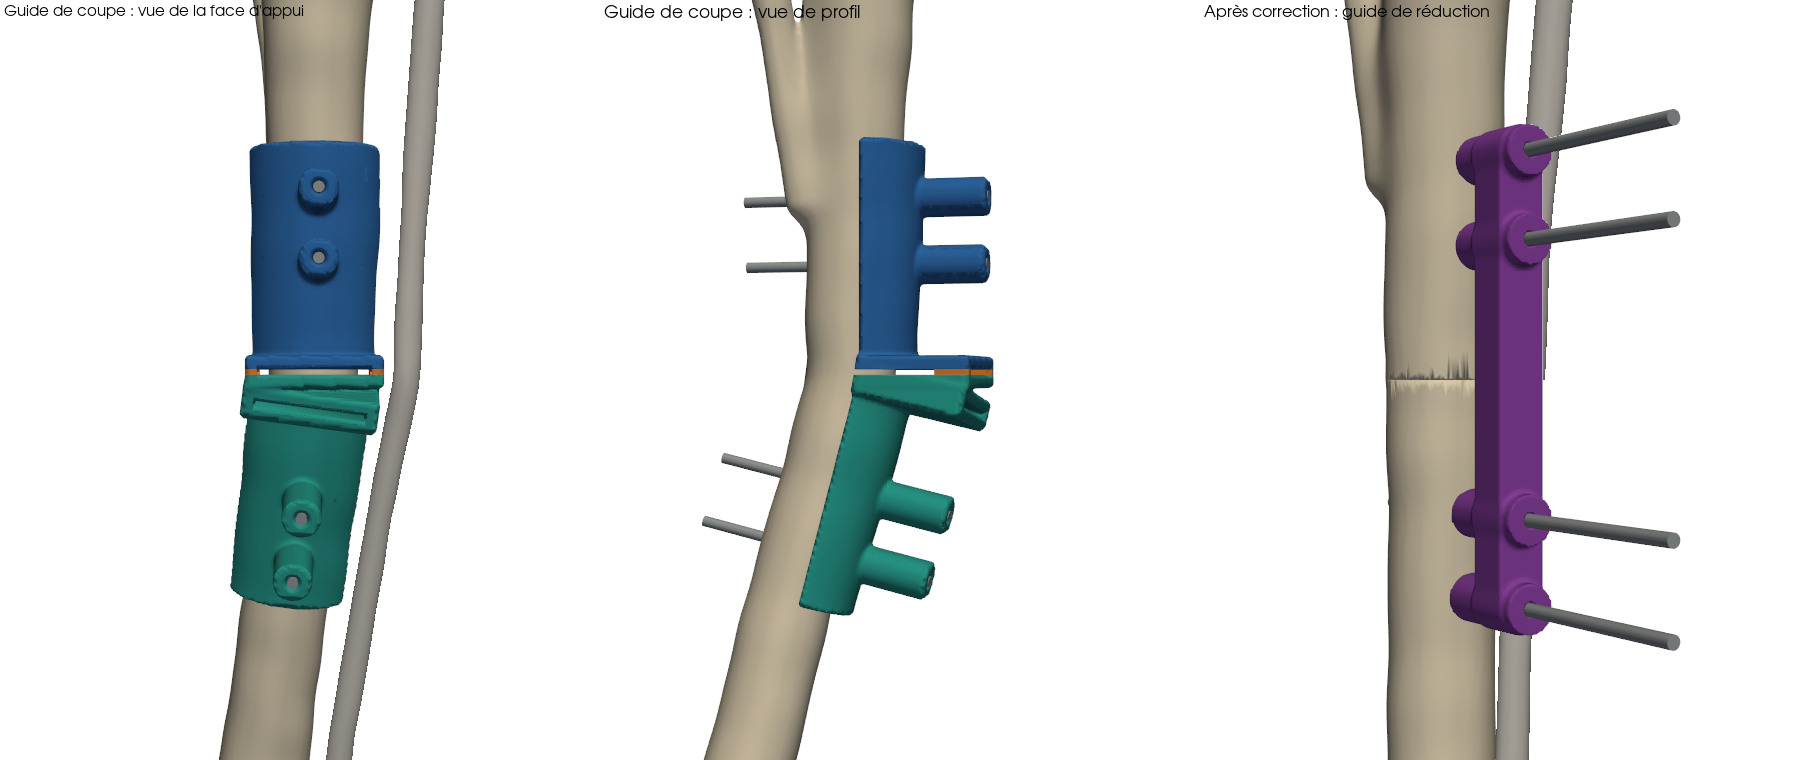
\includegraphics[width=\textwidth]{images/guide_tibia.png}
  \caption{Guide de coupe (bleu et vert) et guide de réduction (violet) d'un tibia.}
  \label{fig:guide}
\end{figure}

\begin{figure}[h]
  \centering
  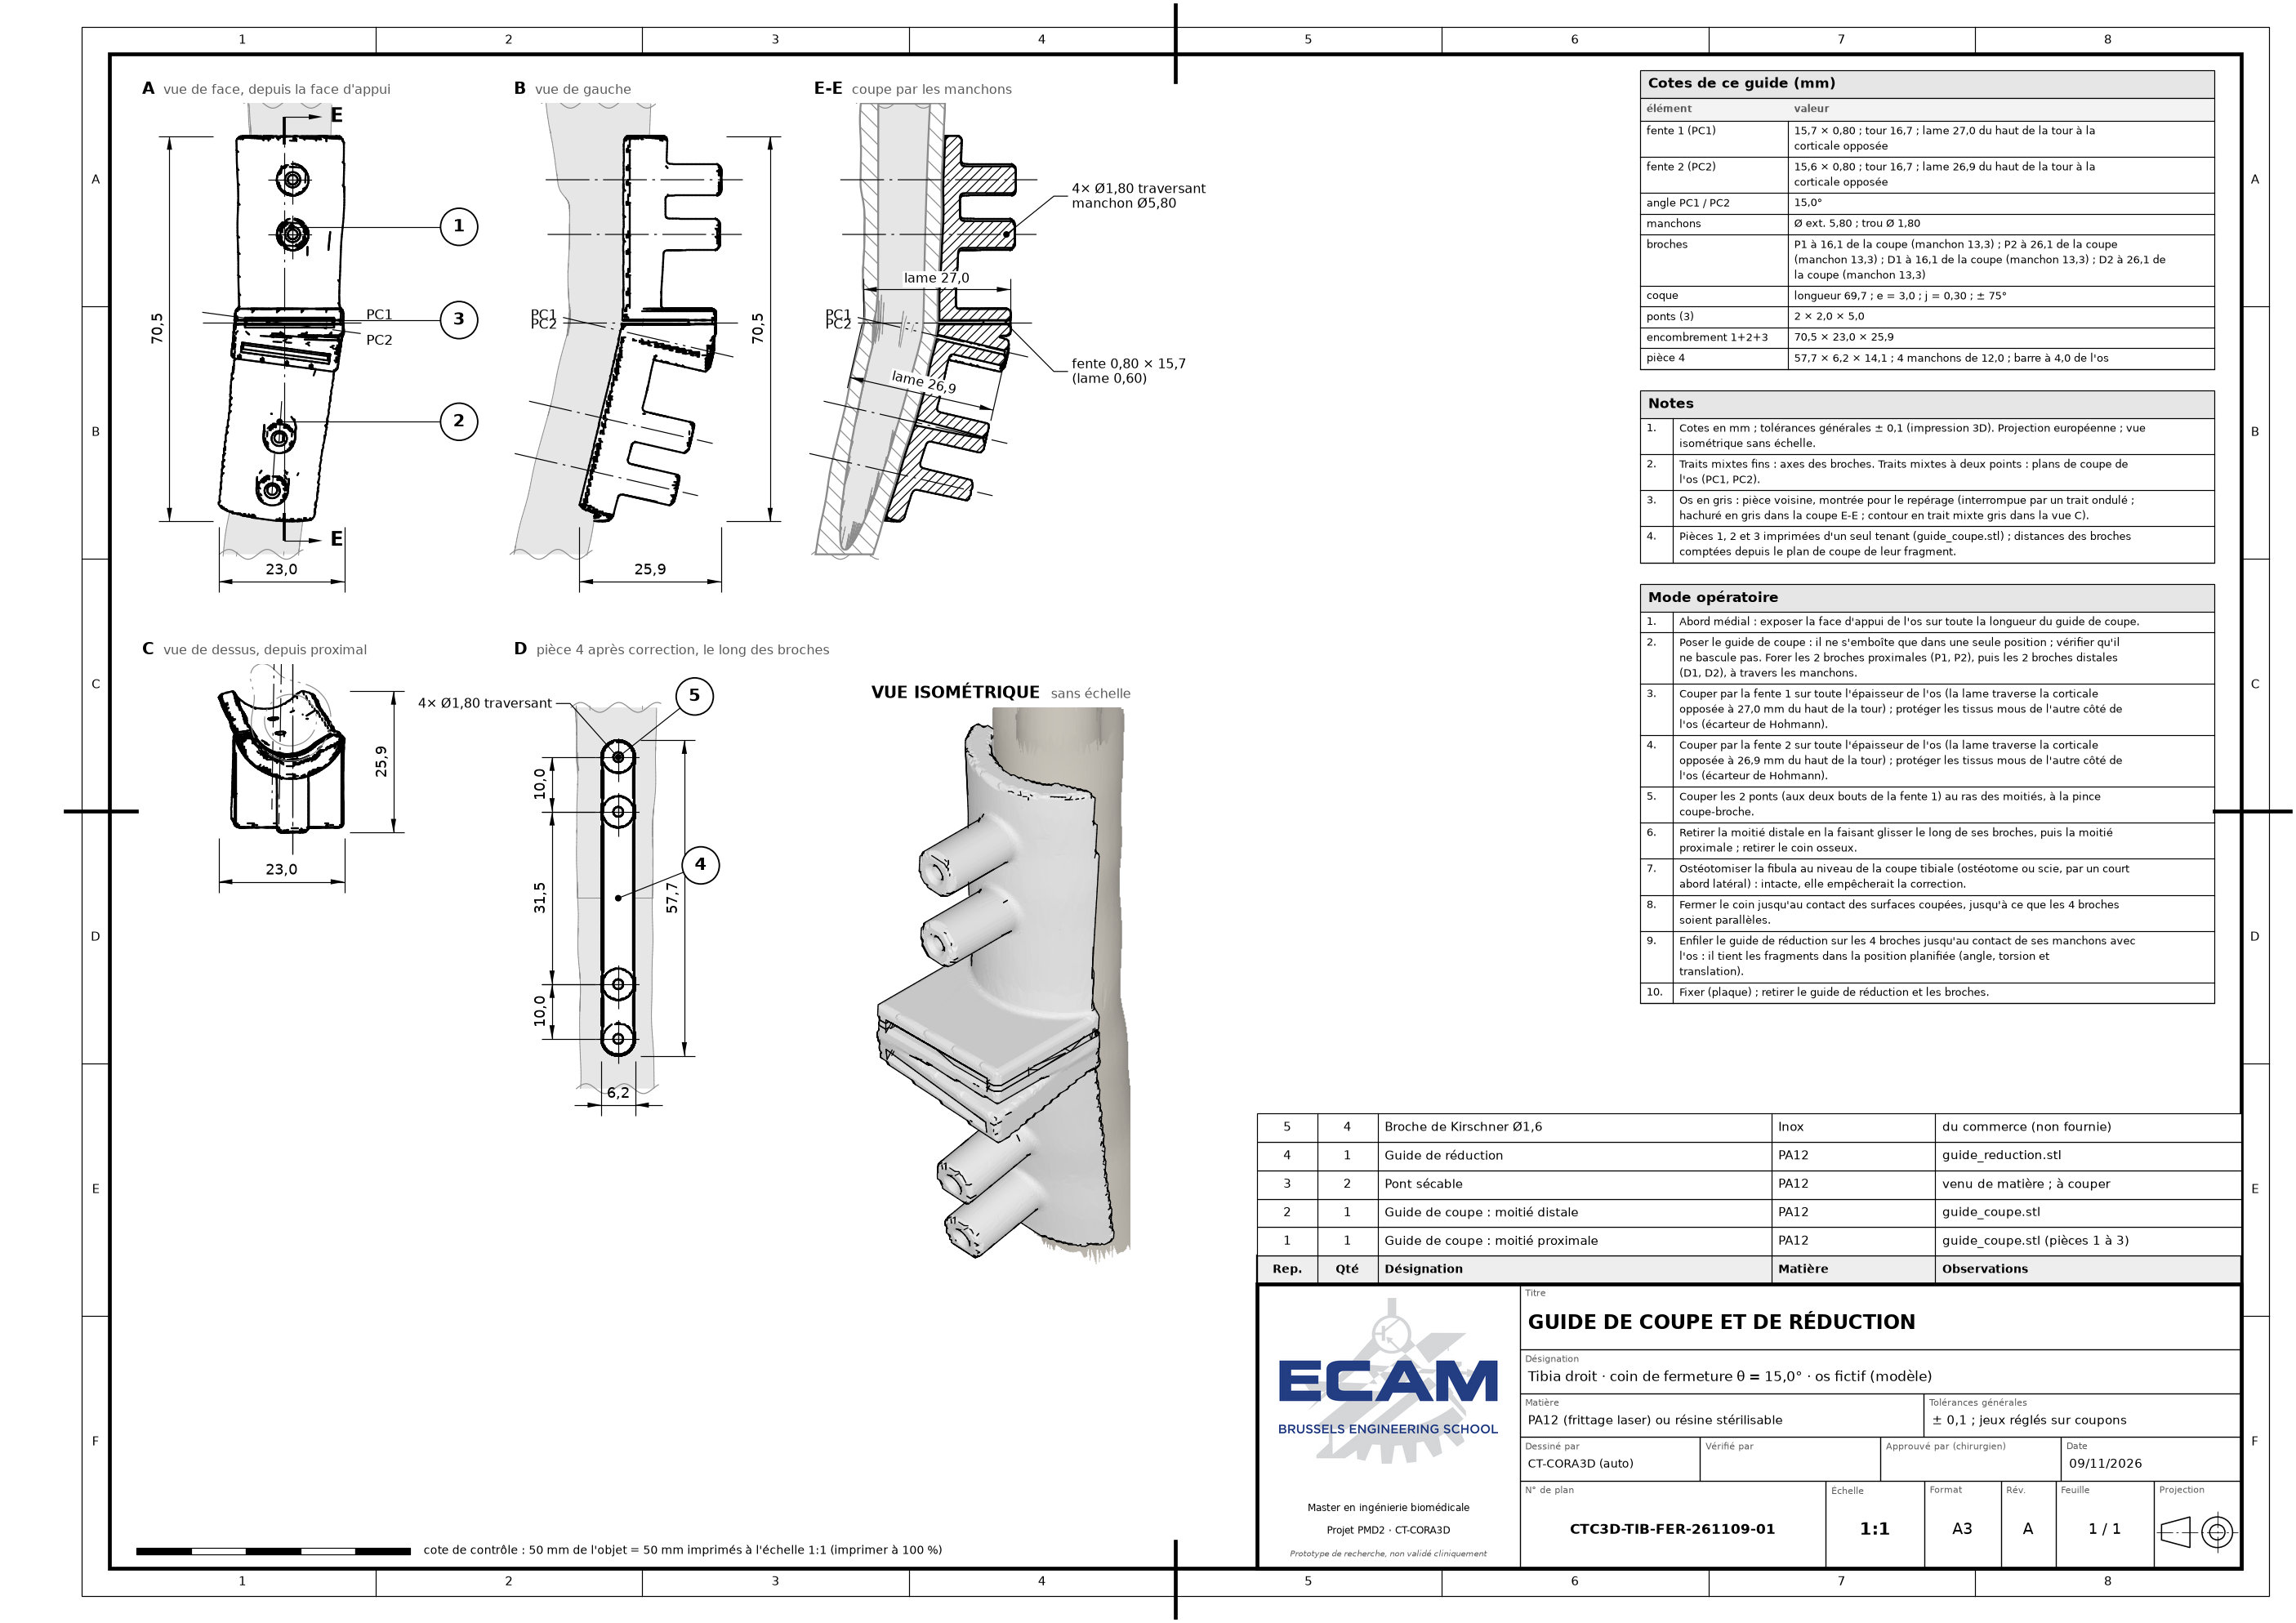
\includegraphics[width=0.9\textwidth]{images/plan_guide_tibia.png}
  \caption{Plan 2D coté du guide, généré automatiquement.}
  \label{fig:plan}
\end{figure}

% ------------------------------------------------------------------ 8
\section{Livrables}

\begin{enumerate}
  \item L'application CT-CORA3D (code source et application installable).
  \item Les guides imprimables (STL) et leurs plans 2D pour les cas étudiés.
  \item Un rapport technique et une présentation orale.
\end{enumerate}

% ------------------------------------------------------------------ 9
\section{Planning}

\begin{tabularx}{\textwidth}{@{}lXl@{}}
\toprule
\textbf{Phase} & \textbf{Contenu} & \textbf{Échéance} \\ \midrule
1 & Lecture DICOM, segmentation, maillages & \textit{(date)} \\
2 & Repères anatomiques et mesures & \textit{(date)} \\
3 & Planification CORA 3D & \textit{(date)} \\
4 & Conception des guides et plans 2D & \textit{(date)} \\
5 & Cas réels, validation, rapport & \textit{(date)} \\
\bottomrule
\end{tabularx}

% ------------------------------------------------------------------ 10
\section{Risques}

\begin{tabularx}{\textwidth}{@{}XX@{}}
\toprule
\textbf{Risque} & \textbf{Mesure prévue} \\ \midrule
Segmentation fausse (os collés, scanner de mauvaise qualité) & Correction manuelle possible dans l'interface \\
Valeurs normales différentes selon la race & Choix de la référence (publications, race) dans l'interface, validation vétérinaire \\
Guide impossible à poser & Refus automatique et proposition d'un autre type de coin \\
Erreur d'impression 3D & Contrôle du jeu sur une pièce test \\ \bottomrule
\end{tabularx}

\end{document}
